%!TEX root = Main.tex
\section*{Linear Classification}
In linear classification the decision surfaces are linear functions of the input vector $\mathbf{x}$.
the target of the classification is labelled in the target variable $\mathbf{t}$, using the target values to represent class labels.
In this project there are 3 different speakers, $K = 3$ then the target vector for class 3 be $\mathbf{t} = (0, 0, 1)^T$.
The value of $t_k$ can be interpreted as the probability of the given class being class $C_k$.
To assign each vector $\mathbf{x}$ with a specific class.
The linear discriminant function in its simplest form
\begin{equation}
y(\mathbf{x}) = \mathbf{w}^T \mathbf{x}+w_0
\label{eq:lin_output}
\end{equation}

\subsection*{Training}
The linear classifier is applied to the training dataset, containing feature vectors $(\mathbf{x}_n)$ and the target vectors $(\mathbf{t}_n)$.
The vectors are on the form:
\begin{equation}
\mathbf{\tilde{X}}=\left[ \begin{array}{c}\mathbf{x}_1^T \quad 1\\
\mathbf{x}_2^T \quad 1\\
...\\ 
\mathbf{x}_n^T \quad 1 \end{array} \right],
\;
\mathbf{T}=\left[ \begin{array}{c}
\mathbf{t}_1^T\\ 
\mathbf{t}_2^T\\ 
...\\
\mathbf{t}_n^T
\end{array} \right]
\label{eq:linearVectors}  
\end{equation} 

This calculation are done to determine the $\tilde{\mathbf{W}}$:
\begin{equation}
\tilde{\mathbf{W}} = \tilde{\mathbf{X}}^\dagger \mathbf{T} \approx  (\tilde{\mathbf{X}}^T \tilde{\mathbf{X}}+\mathbf{I})^{-1} \tilde{\mathbf{X}}^T\mathbf{T}
\label{eq:weightVector}  
\end{equation}
The resulting parameter matrix $ \tilde{\mathbf{W}} $ was tested using the test set.
\begin{equation}
\mathbf{y}(\mathbf{x})=\tilde{\mathbf{W}}^T \tilde{x}, \qquad \tilde{x}= \left[ 
\mathbf{x} \quad 1 
\right]
\end{equation}
The most likely class for each of the feature vectors is found as the index corresponding to the largest value in $ \mathbf{y} $.

\subsection*{Results}

\begin{figure}[H]
\centering
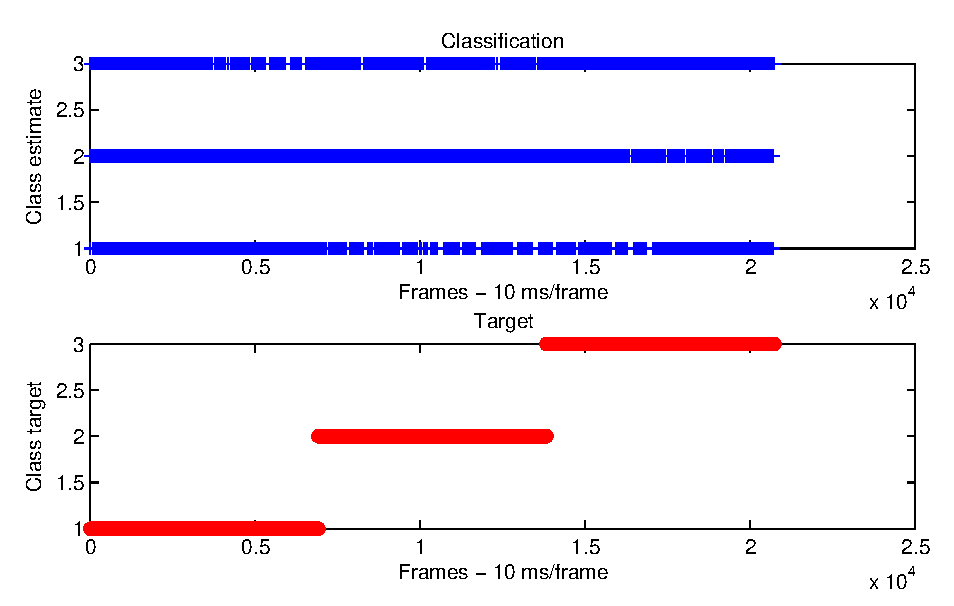
\includegraphics[width=\linewidth]{Linear_1digit_8cent_3speak}
\caption{Results of using linear classifiers and single digit spoken}
\label{fig:Lin_fig_1}
\end{figure}

The result of the linear classifier is a total accuracy of 55.9, 51.2 and 50.6 \% respectively for one, two and ten digits. 
